One of the most important initial goals of \flux\ is to gain
a fundamental understanding of key design challenges pertaining
to the major shift in the new RM conceptual model.
In the context of \flux's run-time system, the scalability
and productivity
challenges---as described in Section~\ref{sect:challenges}---are especially
relevant and crucial. Clearly, we  must provide a wide range
of run-time elements such as parallel programming models,
tools and middleware with performance, scalability, easy integration
and interoperability.
This section evaluates our prototype's performance
and scalability characteristics as well as its ability
to support various HPC run-time elements.


\subsection{KVS Access Patterns (KAP) Tester}
To examine the performance of \flux's run-time system,
we developed a tester called KVS Access Patterns (KAP).
\begin{figure}
  \centering
  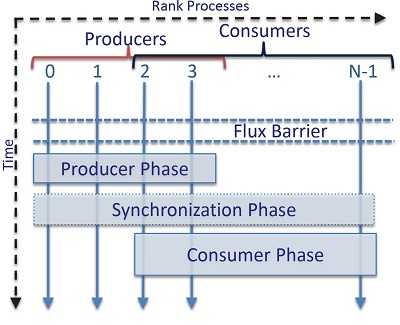
\includegraphics[scale=0.45]{kaptester}
  \caption{Main phases of KAP tester}
  \label{fig:kap}
\end{figure}
KAP models KVS access patterns through various interactions
between KVS writers and readers. Writers are called producers;
readers consumers.
In essence, KAP allows a configurable number of producer processes
to write key-value objects into our KVS 
and a configurable number of consumers to read these
objects after ensuring the consistent KVS state.

In addition to producer and/or consumer counts,
KAP provides a range of parameters that can affect performance.
Among them include the value size (of key-value objects),
the number of objects to put,
the number of objects to read, objects access 
patterns (through different striding), and
synchronization primitives used for consistency.

Figure~\ref{fig:kap} shows the three main phases of KAP.
Right after tester processes are launched into a set of nodes
in which a CMB session had been established,
they are assigned to ranks such that consecutive rank
processes are distributed to consecutive nodes.
Then, the rank processes determine their roles based
on the command line arguments and issue a named barrier
that \flux\ provides to begin to play their roles
simultaneously.

Next, each producer calls the specified number of
{\tt kvs\_put}s of an object of the specified value size.
For each call, the producers use unique keys, but
the values can be configured to be either unique
or redundant.
Once this producer phase completes, all of the producers and consumers
participate in a consistency protocol that uses
\flux's synchronization primitives such as the collective
fence---i.e., the {\tt kvs\_fence} function.
Finally, during the consumer phase, consumers read
these key-value objects by calling {\tt kvs\_get}s.
KAP provides options to emulate various read access
patterns.

